% (The MIT License)
%
% Copyright (c) 2023 Yegor Bugayenko
%
% Permission is hereby granted, free of charge, to any person obtaining a copy
% of this software and associated documentation files (the 'Software'), to deal
% in the Software without restriction, including without limitation the rights
% to use, copy, modify, merge, publish, distribute, sublicense, and/or sell
% copies of the Software, and to permit persons to whom the Software is
% furnished to do so, subject to the following conditions:
%
% The above copyright notice and this permission notice shall be included in all
% copies or substantial portions of the Software.
%
% THE SOFTWARE IS PROVIDED 'AS IS', WITHOUT WARRANTY OF ANY KIND, EXPRESS OR
% IMPLIED, INCLUDING BUT NOT LIMITED TO THE WARRANTIES OF MERCHANTABILITY,
% FITNESS FOR A PARTICULAR PURPOSE AND NONINFRINGEMENT. IN NO EVENT SHALL THE
% AUTHORS OR COPYRIGHT HOLDERS BE LIABLE FOR ANY CLAIM, DAMAGES OR OTHER
% LIABILITY, WHETHER IN AN ACTION OF CONTRACT, TORT OR OTHERWISE, ARISING FROM,
% OUT OF OR IN CONNECTION WITH THE SOFTWARE OR THE USE OR OTHER DEALINGS IN THE
% SOFTWARE.

\documentclass{article}
\usepackage{../painofoop}
\newcommand*\thetitle{Algorithms}
\newcommand*\thesubtitle{History, State, Behavior, Enemies of OOP}
\begin{document}

\plush{\poopTitlePage{1}}

\pptToc

\plush{
    \pptBanner[red]{WARNING!}
    In the pursuit of academic enlightenment within this course, it is paramount to caution that the doctrines disseminated may present a potentially hazardous venture if employed in real-life software projects. This inherent risk arises from the potential incongruity with the broadly accepted canon of object-oriented programming and recognized best programming practices. If one remains resolute in their decision to adapt their coding methodologies to align with the principles propagated in this course, it would be prudent to employ a certain degree of foresight. A humorous, yet sincere suggestion, would be to secure alternate employment prior to a possible premature termination of one's current professional engagement.\par
    \textcolor{gray}{\small Written by me, edited by ChatGPT}
}

\plush{\pptChapter{History}}

\plush{
    \pptSection[Sketchpad]{Who started it?}
    \pptPic{0.5}{ivan-sutherland.png}\\
    Ivan Sutherland's seminal \textbf{Sketchpad} \emph{application} was an early inspiration for OOP, created between 1961 and 1962 and published in his Sketchpad Thesis in 1963. Any object could become a ``master,'' and additional instances of the objects were called “occurrences”. Sketchpad's masters share a lot in common with JavaScript's prototypal inheritance. \textcolor{gray}{(c)~Wikipedia}
}

\plush{
    \pptSection[Objects]{Who invented Objects, Classes, and Inheritance?}
    \pptPic{0.6}{dahl-and-nygaard.jpg}\\
    \textbf{Simula} was developed in the 1965 at the Norwegian Computing Center in Oslo, by Ole-Johan Dahl and Kristen Nygaard. Like Sketchpad, Simula featured objects, and eventually introduced \emph{classes}, class \emph{inheritance}, \emph{subclasses}, and \emph{virtual methods}. \textcolor{gray}{(c)~Wikipedia}
}

\pptSection[Simula-67]{Simula-67: Sample Code}
\begin{ffcode}
Class Figure;
  Virtual: Real Procedure square Is Procedure square;;
Begin
End;
Figure Class Circle (c, r);
  Real c, r;
Begin
  Real Procedure square;
  Begin
    square := 3.1415 * r * r;
  End;
End;
\end{ffcode}
\plush{}

\plush{
    \pptSection[OOP]{Who coined the ``OOP'' term?}
    \pptPic{0.6}{smalltalk-guys.jpg}\\
    \textbf{Smalltalk} was created in the 1970s at Xerox PARC by Learning Research Group (LRG) scientists, including
    Alan Kay, Dan Ingalls, Adele Goldberg, Ted Kaehler, Diana Merry, and Scott Wallace. \textcolor{gray}{(c)~Wikipedia}
}

\pptSection[Smalltalk]{Smalltalk: Sample Code}
{\small\begin{ffcode}
Object subclass: Account [
    |$\vert$| balance |$\vert$|
    Account class >> new [
        |$\vert$| r |$\vert$|
        r := super new. r init. ^r
    ]
    init [ balance := 0 ]
]
Account extend [
    deposit: amount [ balance := balance + amount ]
]
a := Account new
a deposit: 42
\end{ffcode}
}
\plush{}

\plush{\begin{pptMiddle}
    \pptQuote{professor.png}{Everyone will be in a favor of OOP. Every manufacturer will promote his products as supporting it. Every manager will pay lip service to it. Every programmer will practice it (differently). And no one will know just what it is.}{Tim Rentsch, \newline \emph{Object Oriented Programming}, \newline ACM SIGPLAN Notices 17.9, 1982}
\end{pptMiddle}}

\plush{
    \pptSection[Stroustrup]{Who made it all popular?}
    \pptPic{0.7}{bjarne-stroustrup.jpg}\\
    \textbf{C++} was created by Danish computer scientist Bjarne Stroustrup in 1985, by enhancing C language with Simula-like features. C was chosen because it was general-purpose, fast, portable and widely used.\par
    {\small You may enjoy watching this \href{https://www.youtube.com/watch?v=ae6nFZn3auQ}{one-hour dialog} of Dr. Stroustrup and me.}
}

\pptSection[C++]{C++: Sample Code}
\begin{ffcode}
class Figure {
  virtual float square() = 0;
};
class Circle : public Figure {
  Circle(float c, float r) : c(c), r(r) {};
  float square() { return 3.1415 * r * r; };
private:
  float c, r;
};
\end{ffcode}
\plush{}

\plush{\begin{pptMiddle}
    \pptQuote{ole-lehrmann-madsen.jpg}{There are as many definitions of OOP as there papers and books on the topic}{Ole Lehrmann Madsen et al., \newline \emph{What Object-Oriented Programming May Be---And What It Does Not Have to Be}, ECOOP'89}
\end{pptMiddle}}

\plush{
    \begin{pptMiddle}\pptQuote{alan-kay-oopsla.jpg}{I made up the term `object-oriented,' and I can tell you I didn't have C++ in mind}{Alan Kay, OOPSLA'97}\end{pptMiddle}
    \par
    {\small There was an interesting debate between Alan Kay and a few readers of my blog, in the comments section under this blog post:
    \href{https://www.yegor256.com/2017/12/12/alan-kay-was-wrong.html}{Alan Kay Was Wrong About Him Being Wrong}\par}
}

\plush{
\pptSection[Later]{What happened later?}
C++ was released in 1985. And then...\par
\begin{multicols}{2}
Erlang 1986 \\
Eiffel 1986 \\
Self 1987 \\
Perl 1988 \\
Haskell 1990 \\
Python 1991 \\
Lua 1993 \\
JavaScript 1995 \\
Ruby 1995 \\
Java 1995 \\
Go 1995 \\
PHP3 1998 \\
C\# 2000 \\
Rust 2010 \\
Swift 2014
\end{multicols}
}

% \plush{
%     \pptSection[Java]{Who gave us Java?}
%     \pptPic{0.6}{james-gosling.jpg}\\
%     \textbf{Java} was originally developed by James Gosling at Sun Microsystems and released in May 1995.
% }

\plush{\begin{pptMiddle}
    \pptQuote{oscar-nierstrasz.jpg}{There is no uniformity or an agreement on the set of features and mechanisms that belong in an OO language as the paradigm itself is far too general}{Oscar Nierstrasz, \newline \emph{A Survey of Object-Oriented Concepts}, 1989}
\end{pptMiddle}}

\plush{
\pptSection[Features]{Incomplete list of OOP features, so far:}
{\small\begin{pptWide}{4}
Polymorphism \\
Nested Objects \\
Traits \\
Templates \\
Generics \\
Invariants \\
Classes \\
NULL \\
Exceptions \\
Operators \\
Methods \\
Static Blocks \\
Virtual Tables \\
Coroutines \\
Monads \\
Algebraic Types \\
Annotations \\
Interfaces \\
Constructors \\
Destructors \\
Lifetimes \\
Volatile Variables \\
Synchronization \\
Macros \\
Inheritance \\
Overloading \\
Tuple Types \\
Closures \\
Access Modifiers \\
Pattern Matching \\
Enumerated Types \\
Namespaces \\
Modules \\
Type Aliases \\
Decorators \\
Lambda Functions \\
Type Inference \\
Properties \\
Value Types \\
Multiple Inheritance \\
Events \\
Callbacks \\
NULL Safety \\
Streams \\
Buffers \\
Iterators \\
Generators \\
Aspects \\
Anonymous Objects \\
Anonymous Functions \\
Reflection \\
Type Casting \\
Lazy Evaluation \\
Garbage Collection \\
Immutability
\end{pptWide}}
}

\plush{\begin{pptMiddle}
    \pptQuote{edsger-dijkstra.jpg}{Object oriented programs are offered as alternatives to correct ones... Object-oriented programming is an exceptionally bad idea which could only have originated in California.}{Edsger W. Dijkstra, 1989}
\end{pptMiddle}}

\plush{\begin{pptMiddle}
    \pptQuote{linus-torvalds.jpg}{C++ is a horrible language$\dots$ C++ leads to really, really bad design choices$\dots$ In other words, the only way to do good, efficient, and system-level and portable C++ ends up to limit yourself to all the things that are basically available in C.}{Linus Torvalds, 2007 \newline Creator of Linux}
\end{pptMiddle}}

\plush{\begin{pptMiddle}
    \pptQuote{jeff-atwood.jpg}{OO seems to bring at least as many problems to the table as it solves}{Jeff Atwood, 2007 \newline Co-founder of Stack Overflow}
\end{pptMiddle}}

\plush{\begin{pptMiddle}
    \pptQuote{rich-hickey.jpg}{I think that large objected-oriented programs struggle with increasing complexity as you build this large object graph of mutable objects. You know, trying to understand and keep in your mind what will happen when you call a method and what will the side effects be.}{Rich Hickey, 2010 \newline Creator of Clojure}
\end{pptMiddle}}

\plush{\pptThought{The \emph{complexity} of object-oriented code remains its primary drawback}}

\plush{\begin{pptMiddle}
    \pptQuote{asaf-shelly.jpg}{Reading an OO code you can't see the big picture and it is often impossible to review all the small functions that call the one function that you modified}{Asaf Shelly, 2015 \newline \emph{Flaws of Object Oriented Modeling}}
\end{pptMiddle}}

\plush{\begin{pptMiddle}
    \pptQuote{zeba-khanam.jpg}{Object oriented programming promotes ease in designing reusable software but the long coded methods makes it unreadable and enhances the complexity of the methods}{Zeba Khanam, 2018 \newline \emph{Barriers to Refactoring: Issues and Solutions}, International Journal on Future Revolution in Computer Science \& Communication Engineering}
\end{pptMiddle}}

\plush{
    \pptThought{Thus, we don't know anymore what exactly is object-oriented programming, and whether it helps us write better code :(}
    \par
    {\small You can find more quotes in this blog post of mine: \href{https://www.yegor256.com/2016/08/15/what-is-wrong-object-oriented-programming.html}{What's Wrong With Object-Oriented Programming?}}\par
}

\plush{\pptChapter[Intent]{Original Intent}}

\plush{
    \begin{pptMiddle}\pptQuote{david-west.jpg}{The contemporary mainstream understanding of objects (which is not behavioral) is but a pale shadow of the original idea and anti-ethical to the original intent}{David West, \newline \emph{Object Thinking}, 2004}\end{pptMiddle}
    \par
    {\small You may enjoy watching our conversation with Dr. West:
    \href{https://www.youtube.com/watch?v=s-hdZZzMCac}{part I}
    and
    \href{https://www.youtube.com/watch?v=bW5K5cJ-AVs}{part II}.\par}
}

\plush{
    \pptThought{A system is a composition of objects that are abstractions, which hide data and expose behavior*}
    \par
    {\small * This is how I understand the original intent.}
}

\pptSection[Rectangle]{1) What is an ``abstraction''?}
\begin{pptWide}{2}
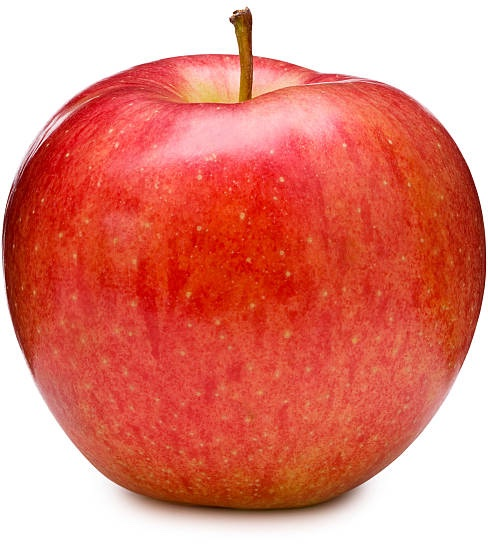
\includegraphics[width=1.3in]{apple.jpg}
\begin{itemize}
\item Color: red
\item Weight: 120g
\item Price: \$0.99
\end{itemize}
\par\columnbreak\par

\includegraphics[width=0.8in]{file-on-disc.jpg}
\par
{\small\begin{ffcode}
var file = {
  path: '/tmp/data.txt',
  read: function() { ... },
  write: function(txt) { ... }
}
\end{ffcode}
}
\end{pptWide}
We deal with an abstraction as if it was a real thing, but eliminating unnecessary details.
We do \ff{file.read()} instead of ``open file handler for data.txt, read byte by byte, store in
byte buffer, wait for the end of file, return the result.''
\plush{}

\pptSection[Rectangle]{How many abstractions are needed?}
\begin{pptWide}{2}
{\small\begin{ffcode}
int square(x1, y1, x2, y2) {
  int w = x2 - x1;
  if (w < 0) { w = w * -1; }
  int h = y2 - y1;
  if (h < 0) { h = h * -1; }
  return w * h;
}
\end{ffcode}
}
\par\columnbreak\par
{\small\begin{ffcode}
int distance(left, right) {
  int d = right - left;
  if (d < 0) { d = d * -1; }
  return d;
}
int square(x1, y1, x2, y2) {
  return distance(x2, x1)
    * distance(y2, y1);
}
\end{ffcode}
}
\end{pptWide}\par
There are two abstractions at the right snippet (``square'' and ``distance''), while only one abstraction at the left one (just ``square'').
\plush{}

\pptSection[Levels]{Levels of abstraction}
\begin{pptWide}{2}
{\small\begin{ffcode}
int distance(left, right) {
  int d = right - left;
  if (d < 0) { d = d * -1; }
  return d;
}
int square(x1, y1, x2, y2) {
  return distance(x2, x1)
    * distance(y2, y1);
}
\end{ffcode}
}
\par\columnbreak\par
\begin{tikzpicture}[line width=2pt]
\node[draw,rectangle,anchor=center] (square) {\texttt{square(3, 9, 13, 2)}};
\node[draw,rectangle,below left=3cm and 0cm of square,anchor=center] (d1) {\texttt{distance(13, 3)}};
\node[draw,rectangle,below right=3cm and 0cm of square,anchor=center] (d2) {\texttt{distance(2, 9)}};
\draw[->] (square) -- (d1);
\draw[->] (square) -- (d2);
\end{tikzpicture}
\end{pptWide}\par
Higher level abstractions must not know and/or rely on semantics of lower level abstractions.
\plush{}

\pptSection[Rectangle]{2) What is ``data hiding''?}
\begin{pptWide}{2}
{\small\begin{ffcode}
f = new File("/tmp/data.txt");
// The data escapes the object! :(
p = f.getPath();
FileUtils.deleteFile(p);
\end{ffcode}
}
\par\columnbreak\par
{\small\begin{ffcode}
f = new File("/tmp/data.txt");
// The boolean data escapes too :)
done = f.delete();
assert(done);
\end{ffcode}
}
\end{pptWide}
\par
Obviously, some data must escape your objects.
\plush{}

\pptSection[Rectangle]{3) What is ``behavior exposing''?}
\begin{pptWide}{2}
This is so called ``anemic'' object:
{\small\begin{ffcode}
var user = {
  login: 'jeff',
  password: 'swordfish',
  age: 32
}
function print(u) {
  console.log(`Hello, ${u.login},
    you are ${u.age} today!`);
}
print(user);
\end{ffcode}
}
\par\columnbreak\par
This object is ``alive'':
{\small\begin{ffcode}
var user = {
  login: 'jeff',
  password: 'swordfish',
  age: 32,
  print: function() {
    console.log(`Hello, ${this.login},
      you are ${this.age} today!`);
  }
}
user.print();
\end{ffcode}
}
\end{pptWide}
\par
\plush{}

\pptSection[Function]{An object as a function}
\begin{pptWide}{2}
{\small\begin{ffcode}
int distance(left, right) {
  int d = right - left;
  if (d < 0) { d = d * -1; }
  return d; }
int square(x1, y1, x2, y2) {
  return distance(x2, x1)
    * distance(y2, y1); }
\end{ffcode}
}
\par\columnbreak\par
{\small\begin{ffcode}
class Distance {
  private int r; private int l;
  Distance(l, r) { l = l; r = r; }
  int value() {
    int d = right - left;
    if (d < 0) { d = d * -1; }
    return d; } }
int square(x1, y1, x2, y2) {
  return new Distance(x2, x1).value()
    * new Distance(y2, y1).value(); } }
\end{ffcode}
}
\end{pptWide}\par
The Java object \ff{Distance} on the right snippet is semantically equivalent to the C function \ff{distance()} on the left one.
\plush{}

\pptSection[State]{Identity, State, Behavior}
\begin{pptWide}{2}
{\small\begin{ffcode}
class Circle {
  private float radius;
  Circle(float r) {
    radius = r; }
  void getRadius() {
    return radius; }
  void setRadius(float r) {
    radius = r; }
  float square() {
    return 3.14 * radius * radius; }
}
\end{ffcode}
}
\par\columnbreak\par
{\small\begin{ffcode}
// Identity:
c1 = new Circle(42.0);
c2 = new Circle(42.0);
c1 != c2;

// State:
c1 = new Circle(42.0);
c2 = new Circle(42.0);
c1.getRadius() == c2.getRadius();

// Behavior:
c1 = new Circle(42.0);
c2 = new Circle(-42.0);
c1.square() == c2.square();
\end{ffcode}
}
\end{pptWide}\par
\plush{}

\pptSection[FigureUtils]{State vs. Behavior}
\begin{pptWide}{2}
{\small\begin{ffcode}
class Circle {
  private float r;
  void setR(float r) { this.r = r; }
  float getR() { return this.r; }
}
class FigureUtils {
  static float calcuateSquare(Circle c) {
    return 3.14 * c.getR() * c.getR();
  }
}
Circle c = new Circle();
c.setR(42.0);
float s = FigureUtils.square(c);
\end{ffcode}
}
\par\columnbreak\par
{\small\begin{ffcode}
class Circle {
  private float r;
  Circle(float r) { this.r = r; }
  float square() {
    return 3.14 * this.r * this.r;
  }
}
Circle c = new Circle(42.0);
float s = c.square();
\end{ffcode}
}\par
How to decide what is \emph{state} and what is \emph{behavior}?
\end{pptWide}
\plush{}

\pptSection[Composition]{4) What is ``composition''?}
\begin{pptWide}{2}
{\small\begin{ffcode}
canvas = new Canvas();
canvas.addCircle(new Circle(42));
canvas.draw();
\end{ffcode}
}
\par\columnbreak\par
{\small\begin{ffcode}
canvas = new Canvas();
circle = new Circle(42);
circle.drawOn(canvas);
\end{ffcode}
}\par
\end{pptWide}
What is composition? What is the ``right'' composition?
\plush{}

\plush{\pptChapter[O.T.]{Object Thinking vs. Algorithms}}

\pptSection[While]{While-Do loop}
\begin{pptWide}{2}
{\small\begin{ffcode}
buffer = []
while true
  c = STDIN.readchar
  break if c == "\n"
  if buffer.length > 3
    STDOUT.puts buffer.join
    buffer = []
  end
  buffer << c
end
\end{ffcode}
}
\par\columnbreak\par
{\small\begin{ffcode}
$ echo 'Hello, world!' |$\vert$| ruby a.rb
Hell
o, w
orld
\end{ffcode}
}
\end{pptWide}
\plush{}

\pptSection[Buffer]{Buffer abstraction}
\begin{pptWide}{2}
{\scriptsize\begin{ffcode}
buffer = []
while true
  c = STDIN.readchar
  break if c == "\n"
  if buffer.length > 3
    STDOUT.puts buffer.join
    buffer = []
  end
  buffer << c
end
\end{ffcode}
}
\par\columnbreak\par
{\scriptsize\begin{ffcode}
class Buffer
  def initialize; @data = []; end
  def push(c)
    if @data.length > 3
      STDOUT.puts @data.join
      @data = []
    end
    @data << c
  end
end
buffer = Buffer.new
while true
  c = STDIN.readchar
  break if c == "\n"
  buffer.push c
end
\end{ffcode}
}
\end{pptWide}
\plush{}

\pptSection[Loop]{Loop abstraction}
\begin{pptWide}{2}
{\scriptsize\begin{ffcode}
class Buffer
  def initialize; @data = []; end
  def push(c)
    if @data.length > 3
      STDOUT.puts @data.join
      @data = []
    end
    @data << c
  end
end
buffer = Buffer.new
while true
  c = STDIN.readchar
  break if c == "\n"
  buffer.push c
end
\end{ffcode}
}
\par\columnbreak\par
{\scriptsize\begin{ffcode}
class Buffer
  # the same
end
class Pull
  def initialize(b); @buf = b; end
  def again
    c = STDIN.readchar
    return false if c == "\n"
    @buf.push c
    true
  end
end
buffer = Buffer.new
pull = Pull.new(buffer)
while pull.again; end
\end{ffcode}
}
\end{pptWide}
\plush{}

\pptSection[Loop]{Loop abstraction}
\begin{pptWide}{2}
{\scriptsize\begin{ffcode}
class Buffer
  # the same
end
class Pull
  def initialize(b); @buf = b; end
  def again
    c = STDIN.readchar
    return false if c == "\n"
    @buf.push c
    true
  end
end
buffer = Buffer.new
pull = Pull.new(buffer)
while pull.again; end
\end{ffcode}
}
\par\columnbreak\par
{\scriptsize\begin{ffcode}
class Buffer
  # the same
end
class Pull
  # the same
end
class Pulls
  def initialize(p); @pull = p; end
  def fetch
    while @pull.again; end
  end
end
Pulls.new(Pull.new(Buffer.new)).fetch
\end{ffcode}
}
\end{pptWide}
\plush{}

\pptSection[Composition]{Object composition}
\begin{pptWide}{2}
{\scriptsize\begin{ffcode}
class Buffer
  def initialize; @data = []; end
  def push(c)
    if @data.length > 3
      STDOUT.puts @data.join
      @data = []
    end
    @data << c
  end
end

class Pull
  def initialize(b); @buf = b; end
  def again
    c = STDIN.readchar
    return false if c == "\n"
    @buf.push c
    true
  end
end

class Pulls
  def initialize(p); @pull = p; end
  def fetch
    while @pull.again; end
  end
end

Pulls.new(
  Pull.new(
    Buffer.new
  )
).fetch
\end{ffcode}
}
\end{pptWide}
\plush{}



\plush{\pptChapter[Enemies]{Enemies of Object Thinking}}

\print{\pptSection[List]{What makes us think as algorithms}}
\print{Global scope (static methods)}
\print{Anemic objects (getters)}
\print{Mutability (setters)}
\print{Workers (``-er'' suffix)}
\print{NULL references}
\print{Type casting (reflection)}
\plush{Inheritance}

\plush{\pptChapter[Exam]{How to Pass the Exam?}}

\print{\pptSection[Project]{Make a software project, which...}}
\print{... is larger than 5,000 lines of functional code,}
\print{... compiles and works,}
\print{... doesn't have static methods,}
\print{... has no getters or public attributes,}
\print{... doesn't use NULL references,}
\print{... has only immutable objects,}
\print{... doesn't use inheritance.}
\plush{Otherwise, just attend 75\% of all lectures and you will get your ``C''.}

\plush{\pptChapter[Literature]{Read and Watch}}

\pptBanner{Read and watch:}

David West, \emph{Object Thinking}, 2004

Yegor Bugayenko, \emph{Elegant Objects}, 2016

Read my 80+ blog posts about OOP, \href{https://www.yegor256.com/tag/oop}{here}

Watch my 15+ lectures about OOP, \href{https://www.youtube.com/playlist?list=PLaIsQH4uc08yw2CsNv5OV30GfKE6XVGii}{on YouTube}

``Object Thinking'' meetup, \href{https://www.youtube.com/watch?v=yT6oO28wEik&list=PLaIsQH4uc08yetzX86w1pPck1QtGEy_ik}{watch on YouTube}.

\end{document}
